\documentclass[11pt, oneside]{article}   	% use "amsart" instead of "article" for AMSLaTeX format
\usepackage{geometry}                		% See geometry.pdf to learn the layout options. There are lots.
\geometry{letterpaper}                   		% ... or a4paper or a5paper or ... 
%\geometry{landscape}                		% Activate for rotated page geometry
%\usepackage[parfill]{parskip}    		% Activate to begin paragraphs with an empty line rather than an indent
\usepackage{graphicx}				% Use pdf, png, jpg, or eps§ with pdflatex; use eps in DVI mode
								% TeX will automatically convert eps --> pdf in pdflatex		
\usepackage{amssymb}

%SetFonts

%SetFonts


%\title{}
%\author{The}
\date{}							% Activate to display a given date or no date

\begin{document}
%\maketitle

\subsection*{Recall}
How to write down a plane passing through a point with a normal vector

\begin{figure}[htbp] %  figure placement: here, top, bottom, or page
   \centering
   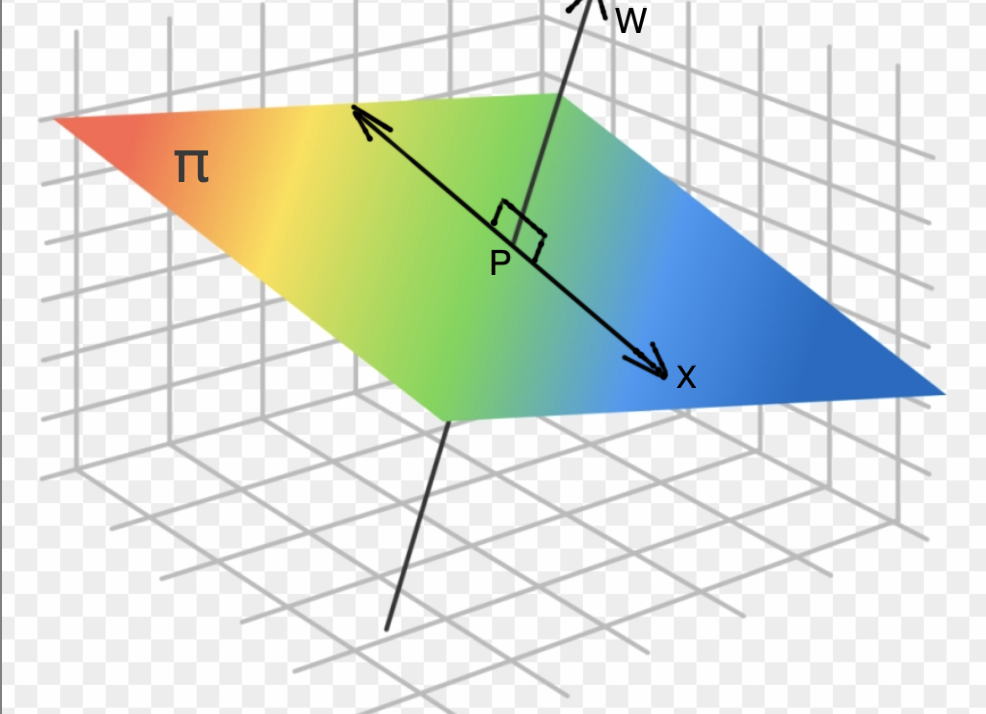
\includegraphics[width=4in]{yyy.png} 
  % \caption{}
   %\label{fig:example}
\end{figure}

\begin{center}
$x$ $\leftrightarrow$ $\vec{ox}$ \\
$p$ $\leftrightarrow$ $\vec{op}$ \\
\end{center}
Write down the characristic of $x \in \pi$  \
\begin{center} $\vec{px} \perp \vec{w}$ \
$\longleftrightarrow$ \ $\vec{px} \cdot \vec{w} = 0$ \\ 
\ $(x-p) \cdot \vec{w} = 0$ \\
$\longleftrightarrow$ $\vec{w} \cdot x - \vec{w} \cdot p = 0$ \\
$\longleftrightarrow$ $\vec{w} \cdot + b = 0$, $\forall x \in \pi$

\end{center}


\end{document}  